
% The environment used here (theappendices) is a wrapper for the basic appendices environment which changes the appearance of the title page and the structure and appearance of the appendices in the table of contents and PDF bookmarks. The original functionality can be restored by simply removing the 'the' from the \begin{} and \end{} statements below.

\begin{theappendices}
    \chapter{Why we need CREPE}
A natural question in the DDSP autoencoder setup is why CREPE is needed.
Deep learning, in most cases, benefits from learning end to end compared to composing multiple models that specialize on subtasks of a complex problem.
Reasons for this can be that human designed subtasks are not the ideal way to break down a problem for neural networks, and that errors made by different components accumulate. \newline
We observe this problem in the DDSP autoencoder as well: if the predicted $f_0$ is not exactly the same as the true $f_0$, the autoencoder has no chance of synthesizing the upper harmonics correctly, which is also discussed in \Cref{mel-mss}. \newline

\section{Spectral Losses Provide Poor Gradients for Learning Pitch}
Instead of using a pretrained model to predict $f_0$, we can also let the encoder output the $f_0$ itself.
Surprisingly, this does not work, and the reason is not an architectural limitation of the encoder.
To proof this, I first evaluated different encoder architectures and found some that can learn to extract the pitch in a supervised fashion using the CREPE output as the ground truth. More details on this can be found in \Cref{supervised-pitch}.
Then, I used the successful architecture in an unsupervised DDSP autoencoder with the same decoder architecture and loss as in the improved baseline.
Note that as $f_0$ is a direct input to the harmonic synthesizer, the meaning of this latent variable as pitch is strictly enforced. 
The trained model does not learn to extract the pitch, and hence cannot learn to reconstruct an audio signal. \newline
This agrees with the findings of \citet{turian_im_nodate}, who show that spectral based losses provide a poor learning signal for unsupervised $f_0$ learning. Concrete, they focus simplified setting of pure sine waves
\begin{equation}
    x_t(f_0, \Phi) = \sin(t f_0 + \Phi)
\end{equation}
and analyze the gradient accuracy, which is defined as the percentage of the times that the gradient points into the correct direction if random values for $f_0, \Phi, \hat{f_0}, \hat{\Phi}$ are used:
\begin{equation}
    P_{f_0, \Phi, \hat{f_0}, \hat{\Phi} \sim \mathcal{U}} [  sign(\frac{\delta}{\delta_{\hat{f_0}}} MSS(x(f_0, \Phi), x(\hat{f_0}, \hat{\Phi}))) = sign(f_0 - \hat{f_0}) ]
\end{equation}
Many spectral based losses like pure $L_1$ distance of a single (not mulitscale) spectrogram or log spectrogram losses have a gradient accuracy of less than 55\%. The MSS performs a bit better with a gradient accuracy of 0.771 if $|f_0 - \hat{f_0}| \to 0 $ and scores above 0.9 if $|f_0 - \hat{f_0}|$ is large.
I repeated these experiments with the MSS, u-MSS and the spectral centroid. \Cref{tab:gradient-accuracy} shows the gradient accuracies, and they are significantly worse than the results reported in \citet{turian_im_nodate} - it is unclear why this is the case, but it supports their main finding even stronger.

\begin{table}
    \centering
    \begin{tabular}{ll}
        MSS & 0.482 \\
        u-MSS & 0.52 \\
        Spectral Centroid Loss & 0.514 \\
    \end{tabular}
    \caption{Gradient Accuracy of Various Loss Functions for Pitch Learning}
    \label{tab:gradient-accuracy}
    \small{For each loss, 1000 pairs of $f_0, \hat{f_0}$ are computed to evaluate the gradient accuracy.}
\end{table}

For the first two, even the global loss landscape that can be seen in \ref{fig:global-loss-landscape} looks quite different than the ideal $L_1$ distance $|f_0 - \hat{f_0}|$.
Since the spectral centroid of a pure sine wave recovers the true $f_0$ exactly up to numerical errors, its global loss landscape looks perfect for learning the pitch.

\begin{figure}
    \begin{tabular}{cccc}
        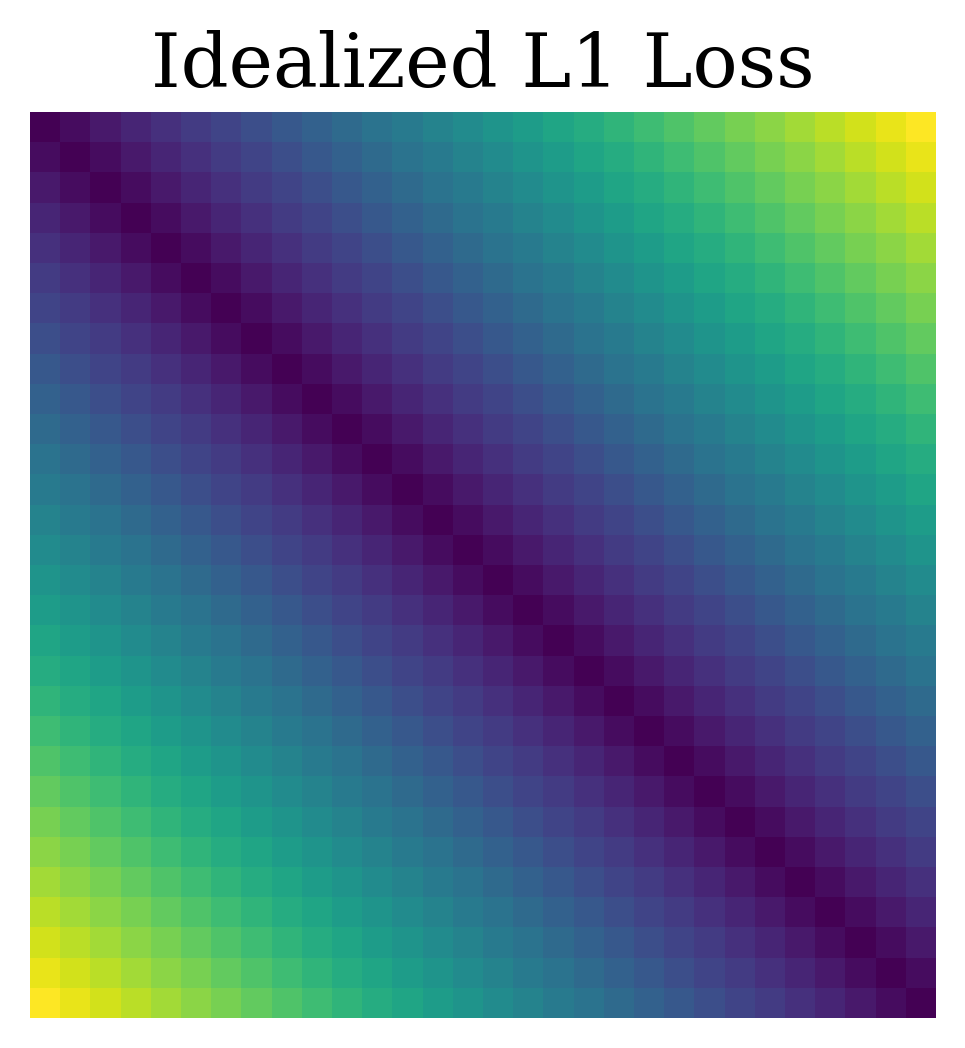
\includegraphics[width=0.24\textwidth]{figures/pitch_learning/global/ideal_l1.png} &
        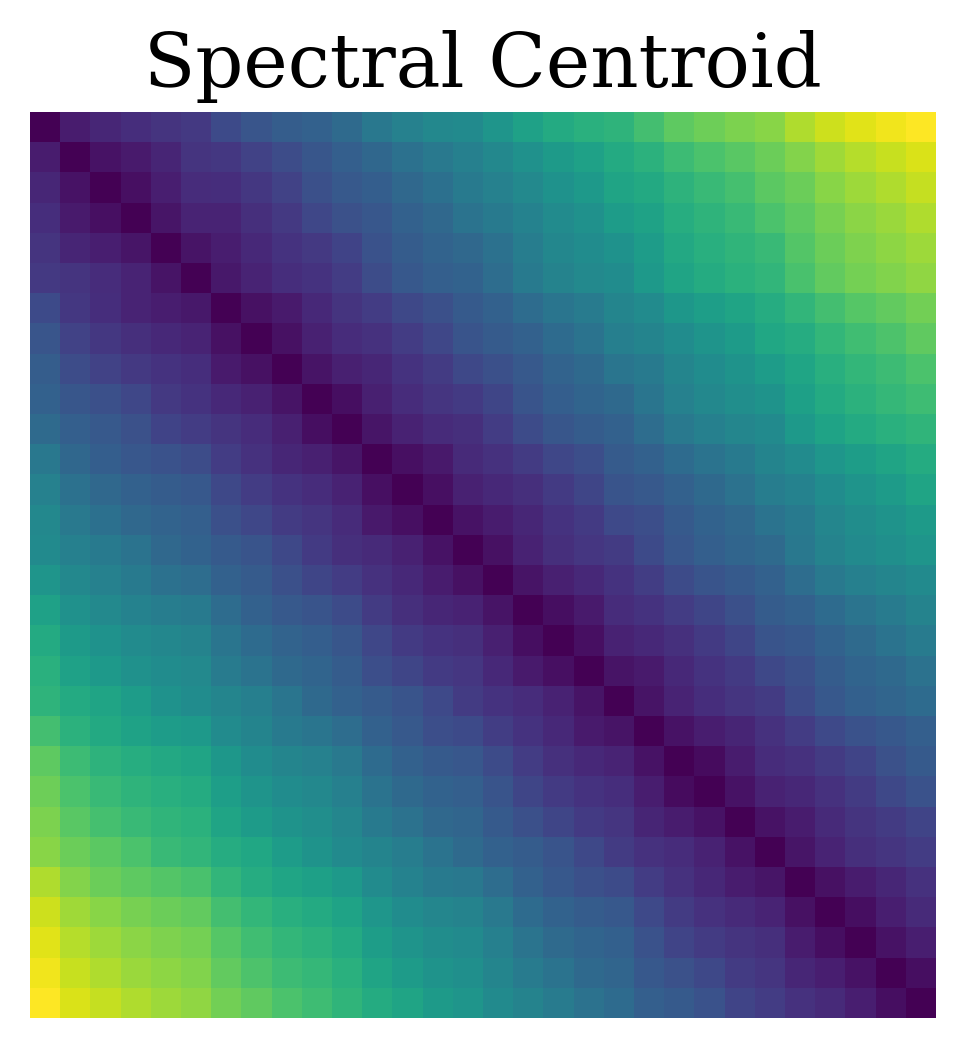
\includegraphics[width=0.24\textwidth]{figures/pitch_learning/global/spectral_centroid.png} &
        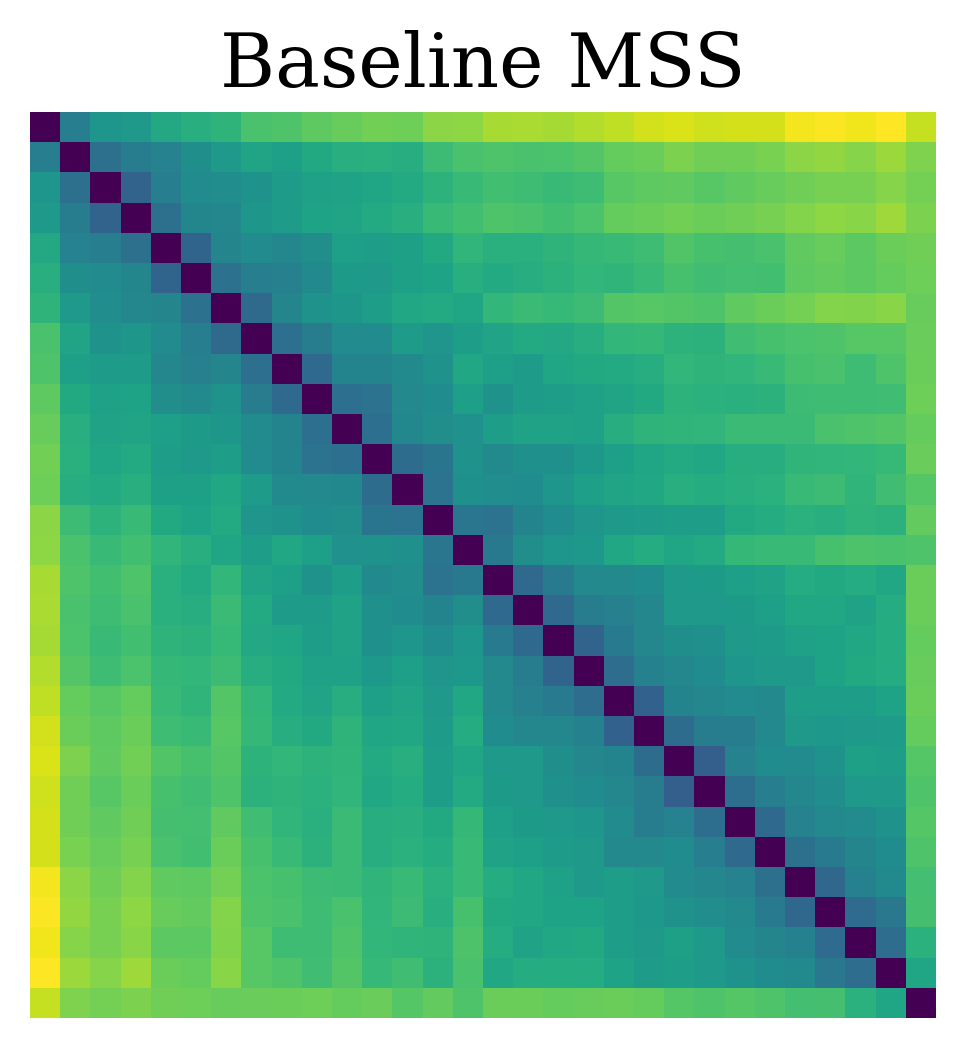
\includegraphics[width=0.24\textwidth]{figures/pitch_learning/global/mss.png} &
        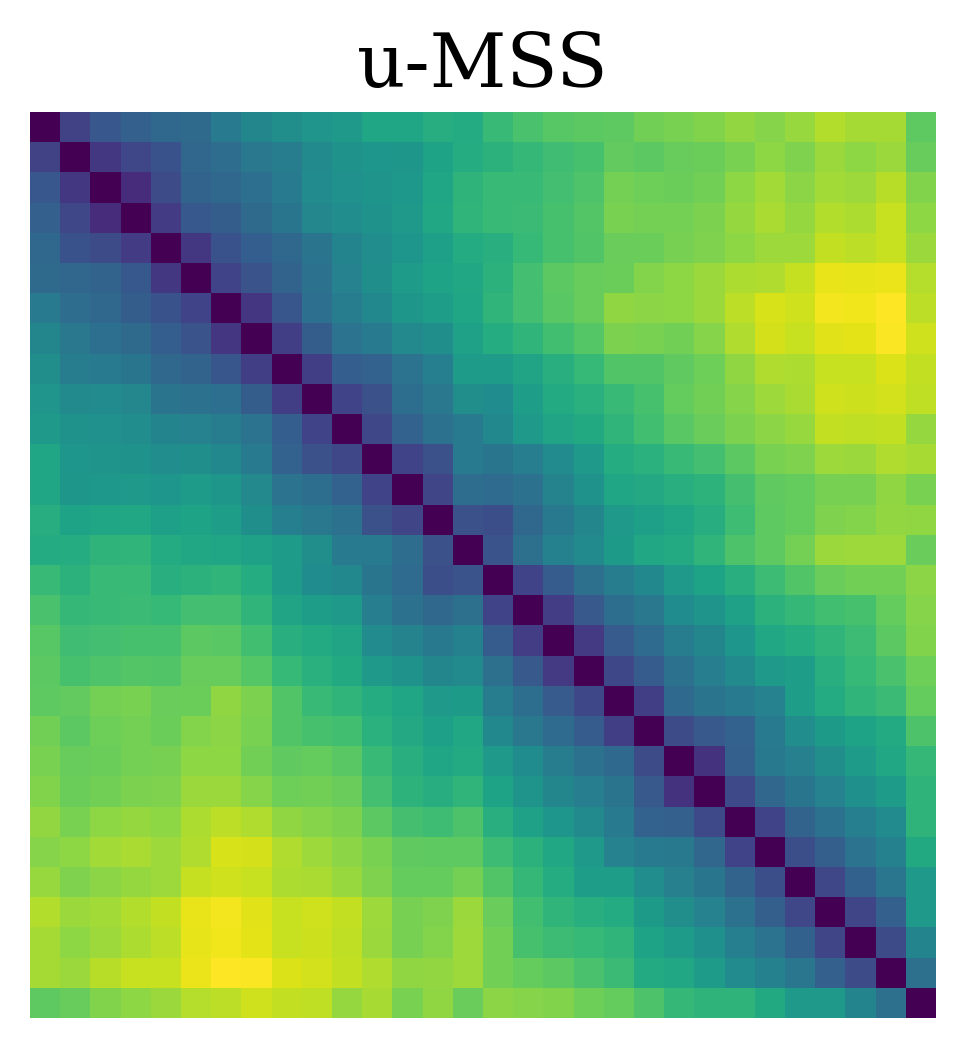
\includegraphics[width=0.24\textwidth]{figures/pitch_learning/global/umss.png} \\
    \end{tabular}
    \caption{Global Loss Landscapes for Pitch Learning}
    \label{fig:global-loss-landscape}
    \small{For each loss, a heatmap shows the error of two sine waves with frequencies according the x- and y-coordinates ranging from 40Hz-100Hz. The ideal loss landscape is plotted simple computes $|x - y|$. This is recovered by the L1 distance of the spectral centroids. The MSS loss and the u-MSS loss have a different global loss landscape, which may hinder pitch learning.}
\end{figure}


However if we plot the gradient $\delta/\delta_{\hat{f_0}} J(x(f_0, \Phi), x(\hat{f_0}, \hat{\Phi}))$, we observe that the gradient oscillates strongly which explains the poor gradient accuracy, see \Cref{fig:oscillating-loss}.
We know that the spectral centroid is exactly correct whenever the frequency can be represented by a single basis vector of the STFT, that is if the resulting spectrogram has a single frequency activation. If we would only consider these points, no oscillation could be observed and the gradient of the spectral centroid would point into the right direction 100\% of the time, as it appears to be the case in \Cref{fig:global-loss-landscape}. However, if the true frequency is somewhere between two basis frequencies, spectral leakage occurs and introduces an error on the gradient. This explains the oscillation observed in \Cref{fig:oscillating-loss} and therefore offers the first explanation for the poor gradient accuracy of spectral losses described in \citet{turian_im_nodate}. \newline
A potential solution that is left for future work is to override the analytical gradient of $f_0$ with a numerically evaluated slope of the loss over a small interval close to the true $f_0$, evaluated only at those frequencies that make up the STFT basis.


\begin{figure}
    \centering
    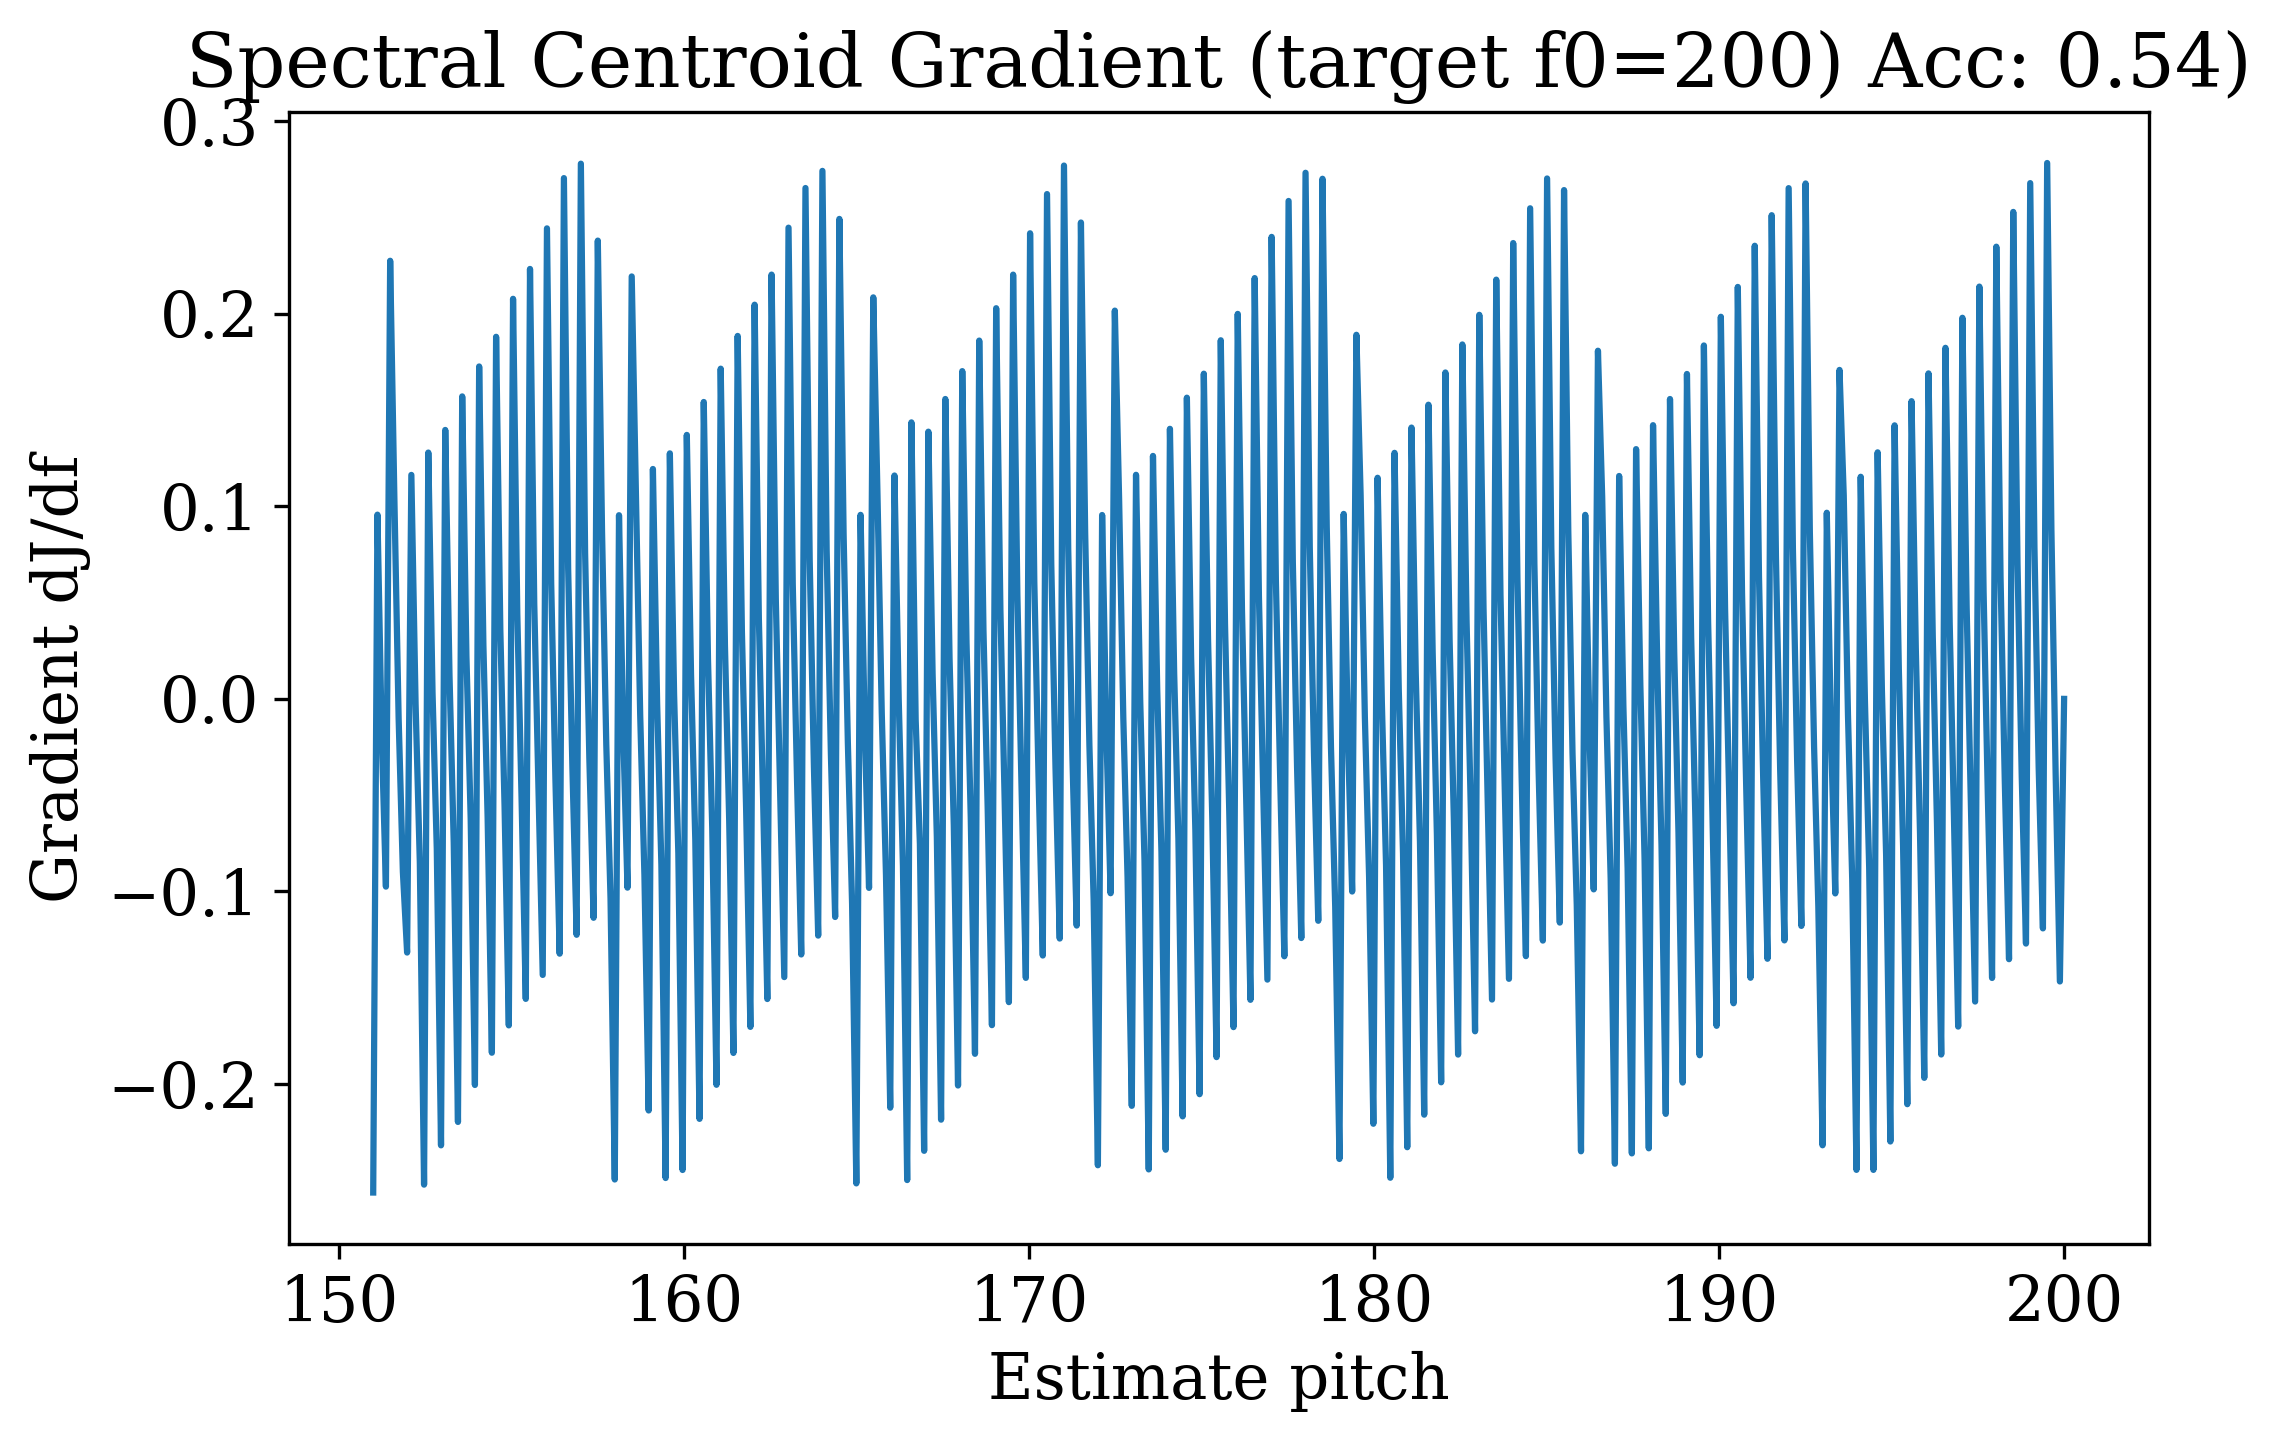
\includegraphics[width=0.5\textwidth]{figures/pitch_learning/oscillation/spectral_centroid_large.png}

    \caption{Oscillating Gradient of $f_0$}
    \label{fig:oscillating-loss}
    \small{For a target signal with $f_0 = 200Hz$, the gradient of the spectral centroid based loss is plotted for varying $\hat{f_0}$ (x-axis). The gradient oscillates strongly and points into the wrong direction almost half the time.}
\end{figure}




\section{Supervised $f_0$ Learning}
\label{supervised-pitch}
% dont use mfccs
% frame it as classification problem
% bam learns super fast
In \citet{ddsp}, an autoencoder that jointly learns to predict $f_0$ and $z$ is trained using a perceptual loss that uses activations of the pretrained CREPE model.
As this approach requires CREPE for training, the encoder can also be trained as a student while CREPE acts as the teacher. \newline
To validate this idea, I searched for an architecture that is able to learn $f_0$ in a supervised manner.
This new model first computes a multiscale spectrogram representation of the input signal as well as MFCCs. The spectrograms are stacked into channels and fed into a stack of convolutional layers. Then, the output is concatenated with the MFCCs and fed to a GRU layer.
The new part of the computational graph involving spectrograms rather than MFCCs is added because MFCCs are designed to be pitch invariant. \newline
CREPE frames the regression problem as a classification problem, where $f_0$ is binned into 360 classes. Indeed, this helps convergence compared to training the model directly with a regression loss like MSE. The classifier is trained using a cross entropy loss, and to evaluate the MAE a weighted mean of the bin centers is computed to obtain $f_0$.
\Cref{fig:supervised-f0-results} shows results for both approaches.

\begin{figure}
    \centering
    \begin{tabular}{ccc}
        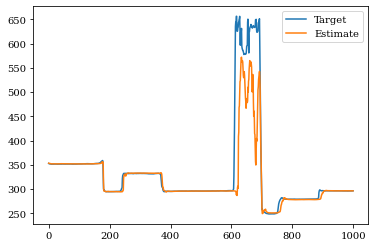
\includegraphics[width=0.31\textwidth]{figures/pitch_learning/supervised/f0_classification_result.png} &
        
        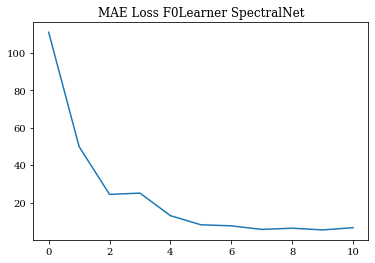
\includegraphics[width=0.31\textwidth]{figures/pitch_learning/supervised/f0_classification_convergence.png}  &
        
        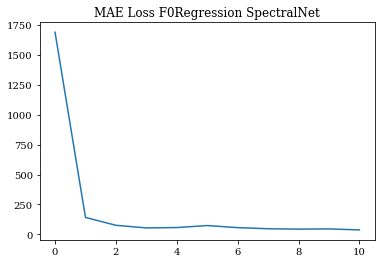
\includegraphics[width=0.31\textwidth]{figures/pitch_learning/supervised/f0_regression_convergence.png} \\
    \end{tabular}
    \caption{Supervised $f_0$ Learning}
    \label{fig:supervised-f0-results}
    \small{\textit{Left:} The prediction of a model trained to predict the correct bin of $f_0$. In the area where the predicted pitch does not align with the true pitch, no audible sound is played. \textit{Center:} Convergence of the Mean Absolute Error (MAE) of the predicted pitch and the true pitch of the same model. \textit{Right:} Convergence of a model with the same architecture, trained directly to optimize the MAE}
\end{figure}

In order to jointly learn $f_0$ and $z$, this model and its training objective can be integrated into the DDSP autoencoder and trained, while the decoder uses the true $f_0$ as an input. During inference, CREPE is then not needed anymore and can be replaced by the estimated $f_0$. Training a DDSP autoencoder in this supervised manner is currently work in progress.


% \section{Jointly Learning $f_0, z$ Using CREPE as Teacher}
% For this section, a DDSP autoencoder is trained just like in \Cref{methods}, with one modification: the encoder architecture is now the same that is used in the previous section with an additional output head for $z$. During training, the decoder uses $f_0$ directly from CREPE, but at the same time the encoder learns  to estimate $f_0$ using the binned classification approach. Once the model has been trained, CREPE is not needed anymore as the encoder learns to predict $f_0$ from the input signal. 
% A sample reconstruction is shown in \Cref{fig:crepestudent-rec}. \newline

% \begin{figure}
%     \centering
%     \begin{tabular}{ccc}
%         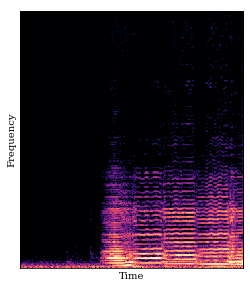
\includegraphics[width=0.31\textwidth]{figures/pitch_learning/joint/true_audio.png} &

%         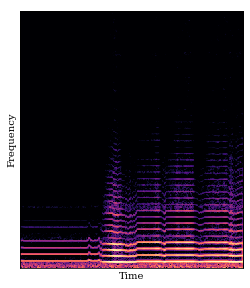
\includegraphics[width=0.31\textwidth]{figures/pitch_learning/joint/reconstructed_audio.png} &
        
%         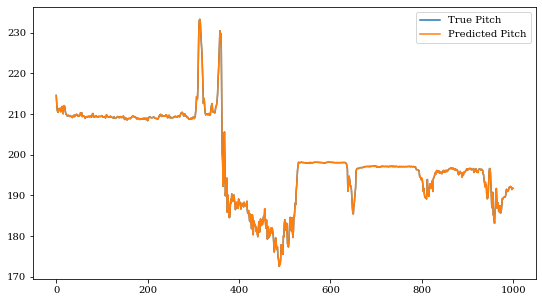
\includegraphics[width=0.31\textwidth]{figures/pitch_learning/joint/reconstructed_pitch.png} \\

%     \end{tabular}
%     \caption{Audio and Pitch Estimation of a CREPE-Supervised Autoencoder}
%     \small{Using CREPE as a teacher to supervise a DDSP autoencoder for learning $f_0$ allows the model to jointly extract $z$ and $f_0$, which is not possible using solely spectral based losses. \textit{Left:} Spectrogram of the original audio. \textit{Center:} Spectrogram of the reconstructed signal. \textit{Right:} Pitch reconstruction}
%     \label{fig:crepestudent-rec}
% \end{figure}

    \label{oscillating-loss}


    \chapter{Interactive Dashboard}
    \label{interactivedashboard}
    For this thesis, a large number of models have been trained and tested on a number of datasets.
    Since subjective evaluation by listening tests remains an important part of finding perceptually good models, a systematic way to find and explore artifacts was needed.
    The interactive dashboard is a web application that allows the user to select a model and a dataset, and then to listen to the model's synthesized audio.
    For this, I implented \href{https://github.com/nielsrolf/pandas\_db}{github.com/nielsrolf/pandas\_db}, which is a key-value-artifact store combined with a web UI to explore data.
    Generated audios, images and metrics can then be searched by their meta data such as model hyperparameters.
    Components of this generic UI are used for the dashboard on \href{https://nielsrolf.github.com?thesis}{nielsrolf.github.com?thesis}.\newline
    It is structured into sections accompaning the methods part of this thesis, and each section displays a comparison of a subset of the trained models.
    In the top part, the user can specify model parameters such as the dataset it has been trained on or which $z$-aggregation has been used, an example is shown in \Cref{fig:screen1}. Since the models have been evaluated on multiple test datasets, the user can additionally select for which one to display metrics and artifacts. \newline
    Below this selection, plots that display the unskewed MSS test losses  and the cycle-reconstruction loss are displayed. In these plots, different model parameters can be compared by selecting multiple configurations in the dropdown menus. \newline
    Below these plots, the user can listen to the synthesized audio and look at generated plots associated with these models and some audio inputs, this is shown in \Cref{fig:screen2}.
    The filters work such that all selected filters must be true and some selections lead to an empty screen. In that case, the user should remove some of the applied filters. \newline
    \begin{figure}
        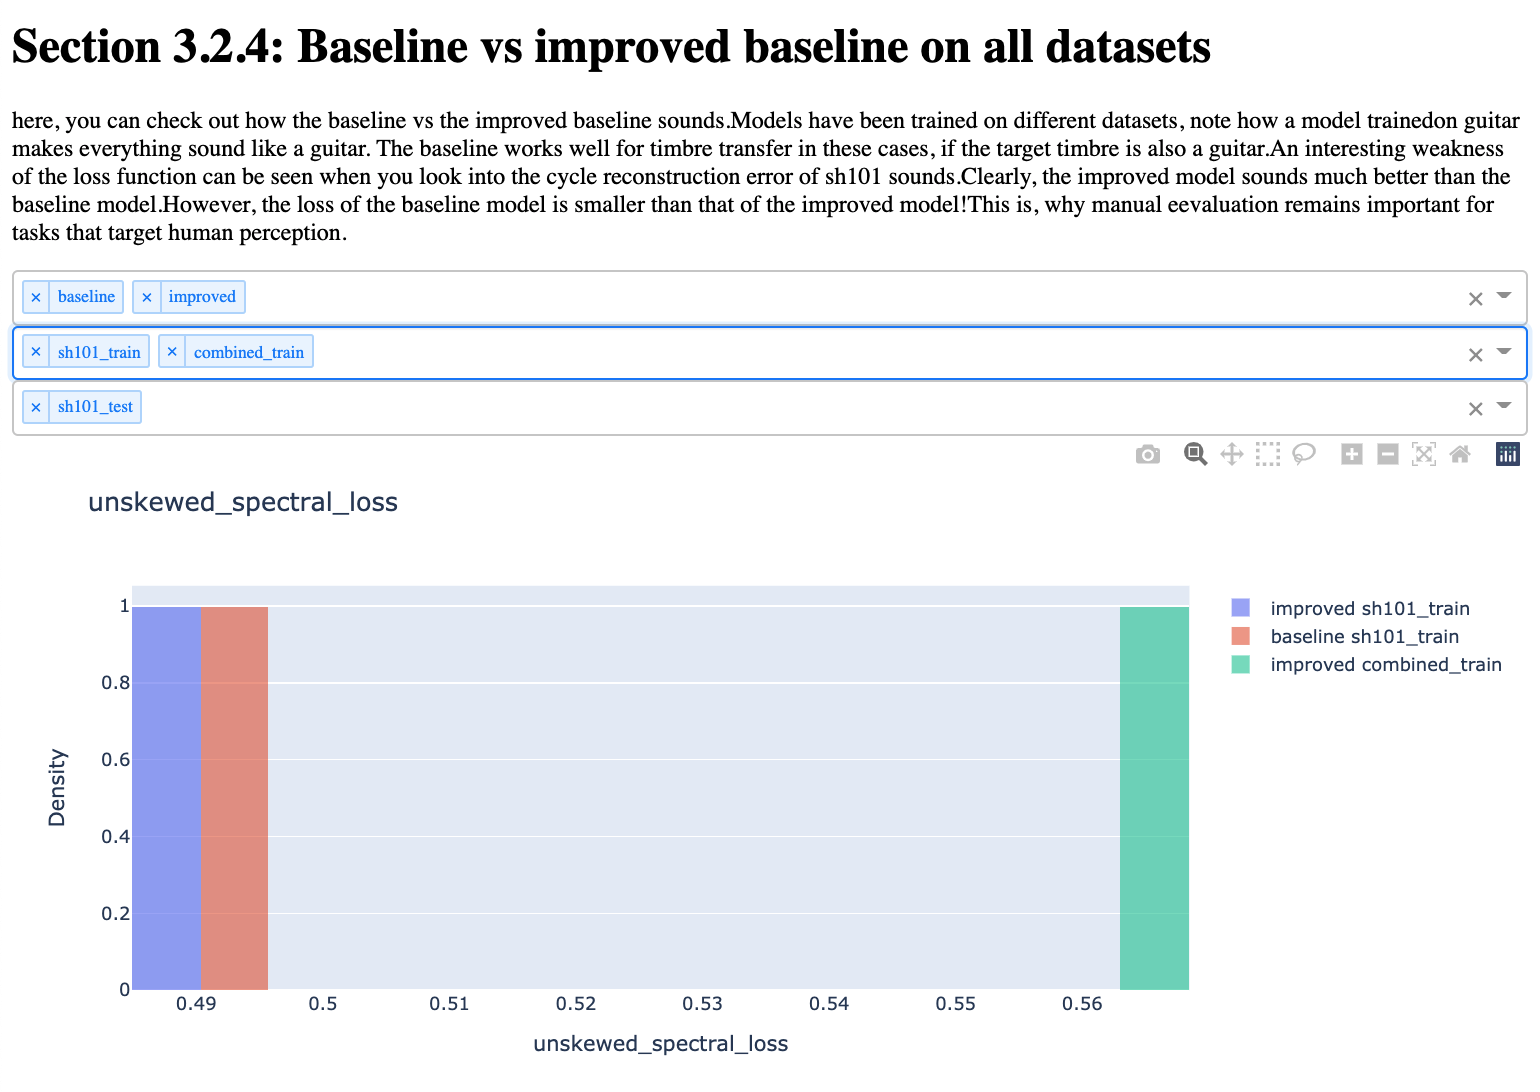
\includegraphics[width=0.9\textwidth]{figures/dashboard/screen1.png}
        \caption{Select parameters of the model and possibly the test dataset}
        \label{fig:screen1}
    \end{figure}
    
    \begin{figure}
        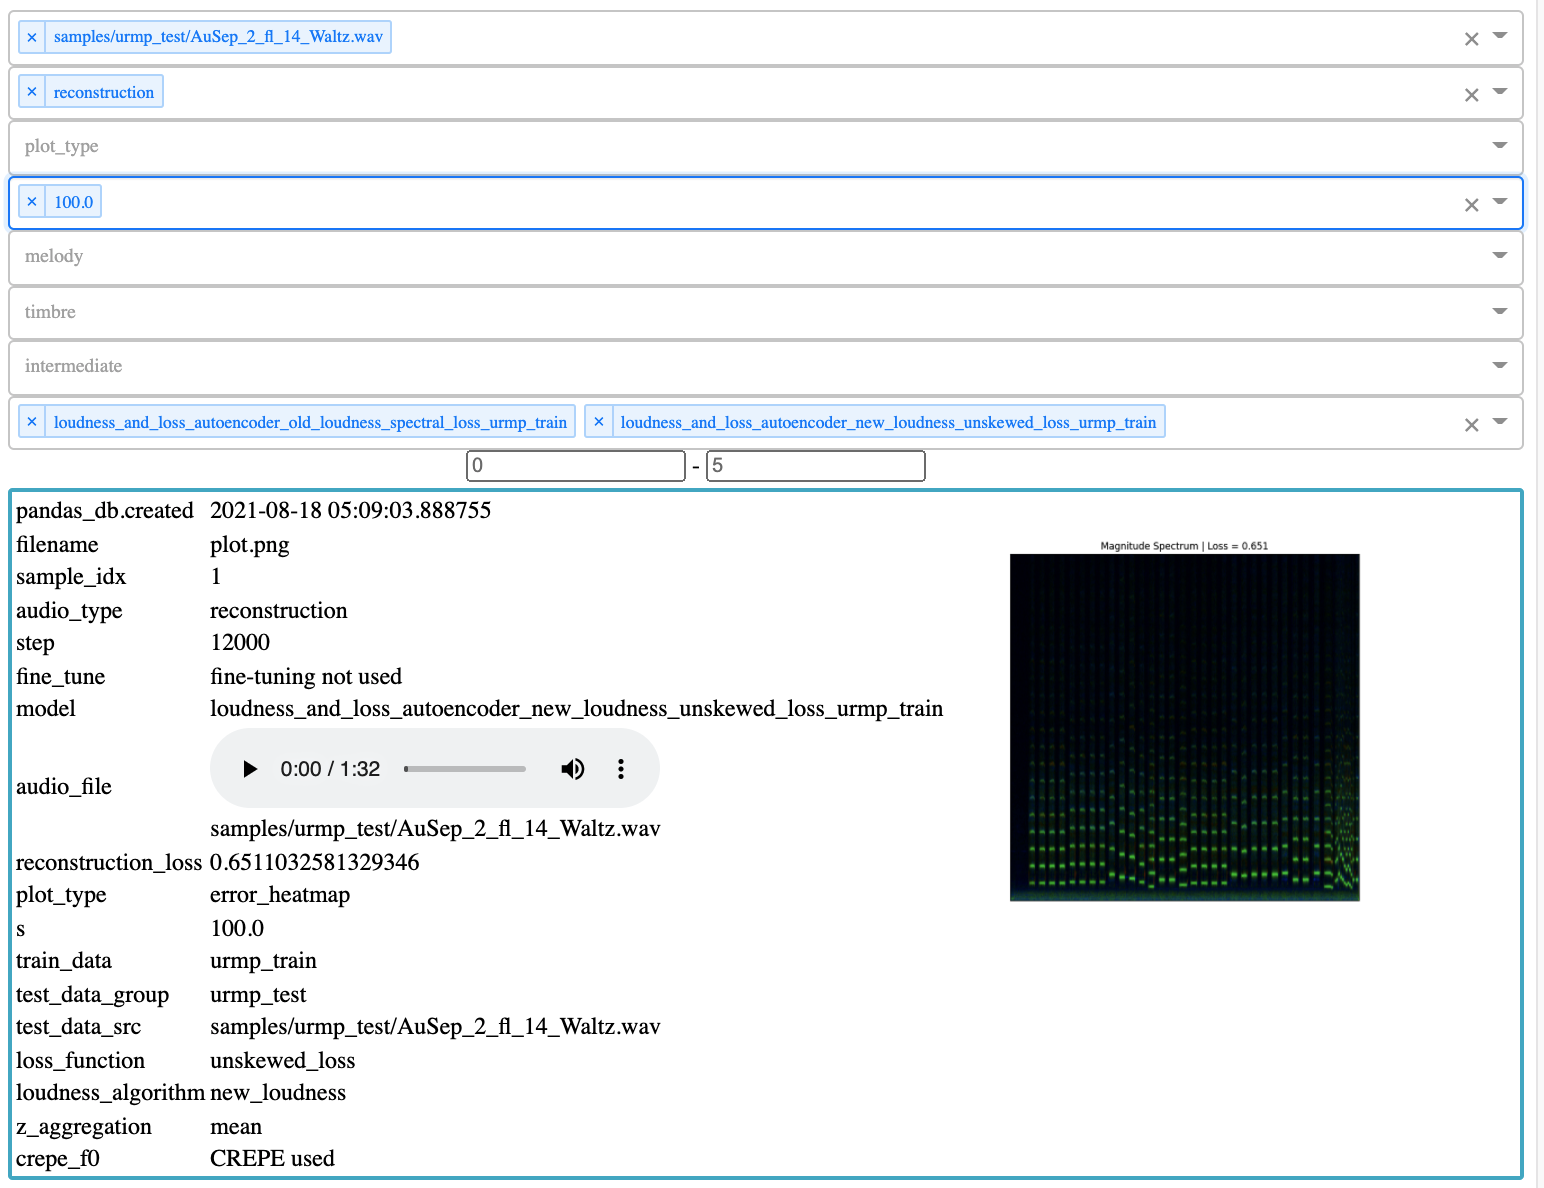
\includegraphics[width=0.9\textwidth]{figures/dashboard/screen2.png}
        \caption{Find reconstructions, timbre transfer audios and cycle reconstructions and compare models}
        \label{fig:screen2}
    \end{figure}

    


\chapter{Training Details}
\label{appendix:trainingdetails}
This section describes the training settings including the model architecture and hyperparameters.
Models have been trained with various settings for the following parameters:
\begin{itemize}
    \item the $z$-aggregation in the encoder
    \item the loudness algorithm
    \item the training loss
    \item the train dataset
\end{itemize}
If not explicitly mentioned, the hyperparameters and architectures described here are therefore used by all models. \newline

\textbf{Preprocessing}
As the very first step, all audio is resampled to 16kHz and converted to mono.
Then, the pretrained CREPE model \citep{kim_crepe_2018} of the official implementation on \href{https://github.com/marl/crepe}{github.com/marl/crepe} is used to extract the pitch contour $f_0$, and the two different versions of the loudness algorithm are applied independently on spectrograms of the audio.
For training, the audio, the pitch contour and the two loudness curves are then cut into slices of 4 seconds with a hop size of 1 second.
During inference, the model can be built for any audio length input and is therefore applied at once to the audio without this additional step.


\textbf{Loudness Algorithm}
The baseline loudness algorithm first computes a spectrogram with a window size of 2048 and 75\% overlap between the windows. Then, it computes:
\begin{equation}
    \begin{split}
    s &= stft(audio) \\
    amp &= |s| \\
    power_{db} &= 20 \quad log_{10}(max(\epsilon, amp)) \\
    loudness &= mean_T(power_{db}+ A_{db})
    \end{split}
\end{equation}
The adjusted loudness algorithm uses a smaller fft size of 512 to achieve a better time-resolution. It computes:
\begin{equation}
    \begin{split}
    s &= stft(audio) \\
    power_{amp} &= |s|^2 \\
    power_{amp}^{+A} &= power_{amp} * A_{amp} \\
    loudness &= 10 \quad log_{10}(max(\epsilon, mean_T(power_{amp}^{+A})))
    \end{split}
\end{equation}

$A$ refers to a constant adjustment factor per frequency - once used in the decibel scale and once used in the amplitude scale. The adjustment factor is taken from the librosa library. \newline
The difference between the two is, that the adjusted version takes the mean in the linear domain and then converts to decibels, while the baseline version takes the mean in the log domain where it is highly sensitive to spectral leakage.


\textbf{Encoder}

The encoder architecture can be divided into a feature extractor and a feature aggregator.
The feature extractor follows the same architecture as the encoder of \citep{ddsp}: in the first step, MFCCs are extracted from the audio signal. Then, instance normalization is applied on the MFCCs and in the second step, the features are passed through a recurrent neural network consisting of one GRU layer and one time-distributed fully connected layer.
In the baseline architecture, this is directly passed to the decoder.
The encoders with mean aggregation simply compute the mean over the time axis without any additional parameters.
The confidence masked $z$-aggregation encoders uses two additional learnable dense layers to predict $\hat{z} \in \mathbb{R}^{(B, T, d)}$ and a confidence mask $c \in \mathbb{R}^{(B, T, d')}$ from the feature extractor output $x$.
Note that the confidence masks dimension $d'$ can be smaller than the dimension of $d$ of $z$ - in early experiments, I experimented with a single confidence value per time step. These models are referenced as 1-d masked in table \Cref{table:trainingdetails}. \newline
\begin{figure}
    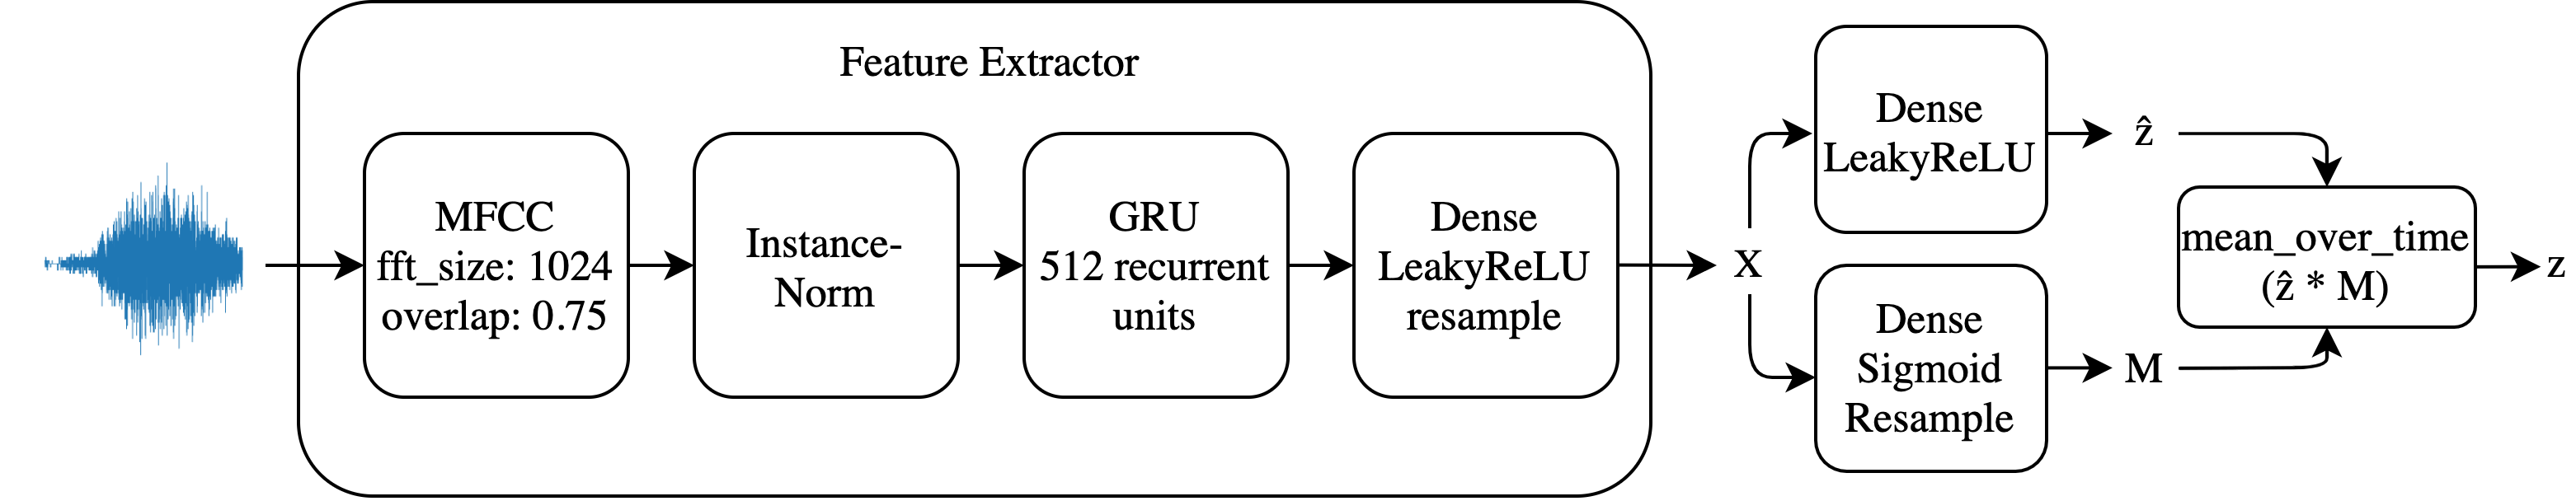
\includegraphics[width=0.95\textwidth]{figures/encoder2.png}
    \caption{Encoder architecture}
    \label{fig:encoder}
\end{figure}
The feature extraction model has 843.852 trainable parameters. If no $z$-aggregation happens or the mean is used, this equals the total number of trainable parameters in the encoder. The confidence masked $z$-aggregation module comes with extra 4104 trainable parameters, or only 513 is the 1d-masked version is used.




% todo schema encoder
% list of layers, output shapes for encoder, aggregator and decoder

\textbf{Decoder}
The decoder gets a normalized loudness and pitch curve as an input and the additional variable $z$ and computes controls for the harmonic synthesizer and the filtered noise synthesizer.
It computes:
\begin{equation}
    \begin{split}
    (ld, f_0, z) & \mapsto (a, h, n) \\
    ld, f_0 &\in \mathbb{R}^{(B, T, 1)} \qquad \text{for us the latent frame rate} \quad T = 1000 \\
    z &\in \mathbb{R}^{(B, T, d)} \qquad \text{in all experiments} \quad d=16 \\
    a &\in \mathbb{R}^{(B, T, 1)}  \qquad \text{amplitude envelope for the harmonic synthesizer} \\
    h &\in \mathbb{R}^{(B, T, 100)}  \qquad \text{harmonic distribution} \\
    n &\in \mathbb{R}^{(B, T, 65)} \qquad \text{noise envelopes for the filtered noise synthesizer}
    \end{split}
\end{equation}

On these three inputs, it applies separate stacks consisting of dense layers and instance normalization. The outputs are then concatenated and passed through a GRU-layer followed by another stack of dense layers with instance normalization. The output is then split into parts that control the filtered noise and the harmonic synthesizer.
In total, it has 6.407.334 trainable parameters.



\textbf{MSS-Loss}
To compute the MSS-loss, magnitude spectrograms with sizes 2048, 1024, 512, 256, 128, 64 have been computed. The baseline MSS-loss computes the $L_1$-distance of those and the corresponding logmag spectrograms.
The adjusted MSS-loss also computes the $L_1$-distance of the magnitude spectrograms and the same spectrograms after passing it through the unskewing function \Cref{eq:unskew} with $s \in \{1, 10, 100\}$.
Before taking the $L_1$-distance, the inputs are scaled to the range $[0, 1]$.

\begin{figure}
    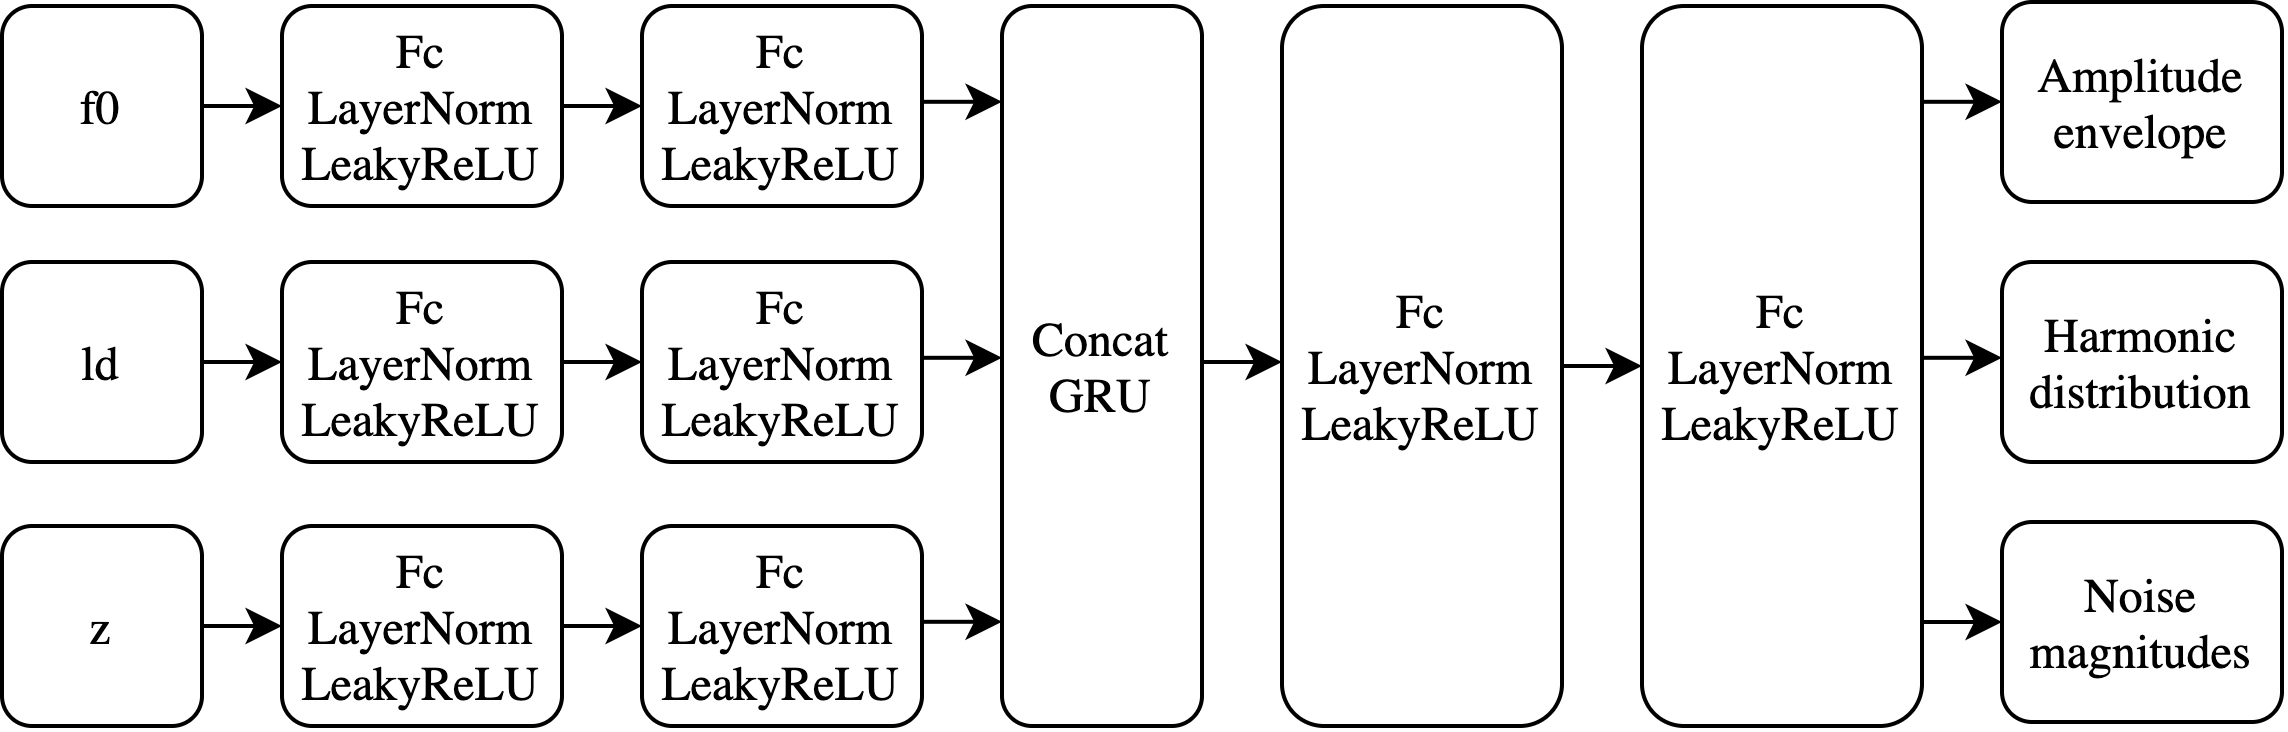
\includegraphics[width=0.9\textwidth]{figures/decoder.png}
    \caption{Decoder architecture}
    \label{fig:decoder}
\end{figure}

\section{Ablation Study Results}
\Cref{table:trainingdetails} shows the full table of results for the ablations studies concerning the changes proposed in \Cref{multi-instrument}. A discussion of the results can be found in \Cref{ablations-summary}

    \begin{longtable}{lllllrr}
        \toprule
     &      &       &          &      &  Reconstruction &  Cycle-Reconstruction \\
Test Data & Train data & Train loss & loudness & z\_aggregation &                 &                       \\
\midrule
bass & bass & baseline & baseline & none &            0.29 &                  1.25 \\
     &      & u-MSS & adjusted & masked &            0.27 &                  0.95 \\
     & combined & u-MSS & adjusted & masked &            0.29 &                  0.90 \\
     & drums & baseline & baseline & none &            0.31 &                  1.00 \\
     & guitar & baseline & baseline & none &            0.45 &                  1.08 \\
     &      & u-MSS & adjusted & masked &            0.39 &                  1.02 \\
     & idmt\_drum & baseline & baseline & none &            0.41 &                  1.17 \\
     &      & u-MSS & adjusted & masked &            0.60 &                  2.29 \\
     & sh101 & baseline & baseline & none &            0.47 &                  0.96 \\
     &      & u-MSS & adjusted & masked &            0.31 &                  0.95 \\
     & urmp & baseline & adjusted & mean &            0.40 &                  0.91 \\
     &      &       & baseline & mean &            0.40 &                  0.97 \\
     &      &       &          & none &            0.34 &                  0.97 \\
     &      & u-MSS & adjusted & 1d-masked &            0.36 &                  0.92 \\
     &      &       &          & masked &            0.36 &                  0.88 \\
     &      &       &          & mean &            0.35 &                  0.92 \\
     &      &       & baseline & mean &            0.34 &                  0.93 \\
combined & bass & baseline & baseline & none &            0.55 &                       \\
     &      & u-MSS & adjusted & masked &            0.49 &                       \\
     & combined & u-MSS & adjusted & masked &            0.26 &                       \\
     & drums & baseline & baseline & none &            0.46 &                       \\
     & guitar & baseline & baseline & none &            0.46 &                       \\
     &      & u-MSS & adjusted & masked &            0.40 &                       \\
     & idmt\_drum & baseline & baseline & none &            0.44 &                       \\
     &      & u-MSS & adjusted & masked &            0.59 &                       \\
     & sh101 & baseline & baseline & none &            0.38 &                       \\
     &      & u-MSS & adjusted & masked &            0.30 &                       \\
     & urmp & baseline & adjusted & mean &            0.42 &                       \\
     &      &       & baseline & mean &            0.47 &                       \\
     &      &       &          & none &            0.43 &                       \\
     &      & u-MSS & adjusted & 1d-masked &            0.36 &                       \\
     &      &       &          & masked &            0.39 &                       \\
     &      &       &          & mean &            0.36 &                       \\
     &      &       & baseline & mean &            0.39 &                       \\
guitar & bass & baseline & baseline & none &            0.67 &                  0.97 \\
     &      & u-MSS & adjusted & masked &            0.58 &                  0.84 \\
     & combined & u-MSS & adjusted & masked &            0.35 &                  0.71 \\
     & drums & baseline & baseline & none &            0.62 &                  0.91 \\
     & guitar & baseline & baseline & none &            0.34 &                  0.83 \\
     &      & u-MSS & adjusted & masked &            0.32 &                  0.66 \\
     & idmt\_drum & baseline & baseline & none &            0.79 &                  1.02 \\
     &      & u-MSS & adjusted & masked &            1.28 &                  2.10 \\
     & sh101 & baseline & baseline & none &            0.46 &                  0.81 \\
     &      & u-MSS & adjusted & masked &            0.43 &                  0.77 \\
     & urmp & baseline & adjusted & mean &            0.49 &                  0.65 \\
     &      &       & baseline & mean &            0.62 &                  0.77 \\
     &      &       &          & none &            0.56 &                  0.89 \\
     &      & u-MSS & adjusted & 1d-masked &            0.39 &                  0.65 \\
     &      &       &          & masked &            0.43 &                  0.67 \\
     &      &       &          & mean &            0.39 &                  0.65 \\
     &      &       & baseline & mean &            0.52 &                  0.79 \\
idmt\_drum & bass & baseline & baseline & none &            0.34 &                  0.76 \\
     &      & u-MSS & adjusted & masked &            0.23 &                  0.67 \\
     & combined & u-MSS & adjusted & masked &            0.12 &                  0.50 \\
     & drums & baseline & baseline & none &            0.19 &                  0.53 \\
     & guitar & baseline & baseline & none &            0.41 &                  0.77 \\
     &      & u-MSS & adjusted & masked &            0.21 &                  0.59 \\
     & idmt\_drum & baseline & baseline & none &            0.10 &                  0.66 \\
     &      & u-MSS & adjusted & masked &            0.11 &                  0.49 \\
     & sh101 & baseline & baseline & none &            0.39 &                  0.65 \\
     &      & u-MSS & adjusted & masked &            0.22 &                  0.56 \\
     & urmp & baseline & adjusted & mean &            0.26 &                  0.62 \\
     &      &       & baseline & mean &            0.27 &                  0.73 \\
     &      &       &          & none &            0.24 &                  0.66 \\
     &      & u-MSS & adjusted & 1d-masked &            0.24 &                  0.65 \\
     &      &       &          & masked &            0.24 &                  0.65 \\
     &      &       &          & mean &            0.23 &                  0.63 \\
     &      &       & baseline & mean &            0.23 &                  0.73 \\
sh101 & bass & baseline & baseline & none &            1.39 &                  1.57 \\
     &      & u-MSS & adjusted & masked &            1.27 &                  1.62 \\
     & combined & u-MSS & adjusted & masked &            0.57 &                  1.58 \\
     & drums & baseline & baseline & none &            1.06 &                  1.46 \\
     & guitar & baseline & baseline & none &            1.02 &                  1.44 \\
     &      & u-MSS & adjusted & masked &            0.97 &                  1.27 \\
     & idmt\_drum & baseline & baseline & none &            1.02 &                  1.64 \\
     &      & u-MSS & adjusted & masked &            1.26 &                  2.42 \\
     & sh101 & baseline & baseline & none &            0.49 &                  1.15 \\
     &      & u-MSS & adjusted & masked &            0.49 &                  1.28 \\
     & urmp & baseline & adjusted & mean &            1.03 &                  1.25 \\
     &      &       & baseline & mean &            1.15 &                  1.31 \\
     &      &       &          & none &            1.09 &                  1.48 \\
     &      & u-MSS & adjusted & 1d-masked &            0.87 &                  1.54 \\
     &      &       &          & masked &            0.95 &                  1.51 \\
     &      &       &          & mean &            0.85 &                  1.47 \\
     &      &       & baseline & mean &            0.91 &                  1.33 \\
urmp & bass & baseline & baseline & none &            0.58 &                  1.31 \\
     &      & u-MSS & adjusted & masked &            0.49 &                  1.10 \\
     & combined & u-MSS & adjusted & masked &            0.37 &                  0.91 \\
     & drums & baseline & baseline & none &            0.42 &                  1.05 \\
     & guitar & baseline & baseline & none &            0.55 &                  1.25 \\
     &      & u-MSS & adjusted & masked &            0.45 &                  0.86 \\
     & idmt\_drum & baseline & baseline & none &            0.66 &                  1.24 \\
     &      & u-MSS & adjusted & masked &            0.84 &                  2.09 \\
     & sh101 & baseline & baseline & none &            0.59 &                  1.01 \\
     &      & u-MSS & adjusted & masked &            0.47 &                  1.00 \\
     & urmp & baseline & adjusted & mean &            0.33 &                  0.81 \\
     &      &       & baseline & mean &            0.34 &                  0.90 \\
     &      &       &          & none &            0.32 &                  0.98 \\
     &      & u-MSS & adjusted & 1d-masked &            0.28 &                  0.81 \\
     &      &       &          & masked &            0.30 &                  0.83 \\
     &      &       &          & mean &            0.29 &                  0.83 \\
     &      &       & baseline & mean &            0.30 &                  0.93 \\
\bottomrule
        
        \caption{Training setting of all models trained}
        \label{table:trainingdetails}
    \end{longtable}



\end{theappendices}